\chapter{Introduction}

\section{Purpose of the Thesis}

This thesis investigates the two research areas \mss{} and
\ogs{}. Both areas have individually been the topic of intense research lately
(\mss{}:\cite{zimmermann2016microservices}, \cite{di2017research},
\ogs{}:\cite{bosch2017towards}, \cite{smed2017algorithms},
\cite{liu2017apparatus}) but very little research exists on how to combine the
two.

In regard to the \mss{} domain this thesis serves as a basis for the discussion
about \ms{} applications. Especially the architecture of such distributed \ms{}
applications is of particular interest. Architecture relevant aspects are
both examined in theory and practically to propose a all-embracing recipe on how
to develop and operate of a \ms{} application. Of particular interest is the
topic of how to facilitate the composition of \mss{} and how to deploy a \ms{}
application in a modern cloud environment.

Another goal of this thesis is to provide proof of concept that it is possible
to develop \ogs{} using \mss{}. For this purpose a vertical slice prototype of a
\ms{} driven \og{} is developed to showcase the necessary fragments that make up
a working \og{} using a \ms{} design. Furthermore this prototype serves as a
simple example of how to reproduce the development process of \ogs{}. The idea
behind the prototype is to make this process simple enough for newcomers in
\og{} development to be understood.


\section{Theoretical framework}

A theoretical framework is being used in order to curtail the infinite amount of
research problems that the topics \ogs{} and \mss{} offer. A theoretical
framework is a \gls{dsm} construct used to frame research problems. \gls{dsm} is
further detailed in \autoref{sub:dsm}.

Within the framework the abstract research problems are gathered and are
translated into research questions that sufficiently cover the area of interest.
According to the research questions hypotheses can be formulated. These
hypotheses are the condensed essence of the research questions and are well
suited for formal verification. The verification of the hypotheses is the
substance of this thesis and contributions to the verification are mentioned at
relevant locations throughout this thesis. Answers to the research questions
are proposed in the concluding \autoref{sub:summary_of_findings}.

\subsection{Research Problems and Research Questions}
\label{sub:problems}

\subsubsection{Usability of a \ms{} for \ogs{}} 

The research problem to examine the usability of \mss{} to develop and operate
an \og{} leads to the following research questions:

\begin{itemize}
  \item Can an \og{} run in a \ms{} environment?
  \item Is a \ms{} influenced architecture suitable to design an \og{}?
  \item Is the added complexity which \ms{} development introduces tolerable
  in comparison to traditional \og{} development?
  \item Do \ms{} applications provide enough performance to drive a fast-paced
  \og{}?
\end{itemize}

\subsubsection{Deployment and Operation}

The problem of deploying and operating a \ms{} driven \og{} application in a cloud
cluster environment raises the following research questions:

\begin{itemize}
  \item What steps are necessary to bring a \ms{} driven \og{} ``from code to
  the cloud''?
  \item How can the deployment process be automated?
  \item How well do \ogs{} run in a cluster environment?
  \item How does a modern container engine assist in deploying and operating a
  \ms{} driven application?
  \item What tools exist that help the developer with the deployment?
\end{itemize}

\subsubsection{\ms{} Composition}
The problem of how to compose of a set of \mss{} to form a coherently
distributed application results in the following research questions:

\begin{itemize}
  \item What degree of composition is necessary for a \ms{} application
  to work?
  \item Which of the two common paradigms of orchestration and choreography is
  better suited for \ms{} composition?
  \item Which middle-ware is most useful in furnishing \ms{} composition?
  \item How can multiple game features be developed parallel within different
  \mss{} while preserving the overall application behaviour?
  \item What problems are introduced by loosely coupling game features?
  \item How does the consistency vs. performance trade-off impact \ogs{}?
  \item What protocols help to reduce service coupling?
\end{itemize}

\subsubsection{\ms{} Development}
The focus on the development process of a \ms{} application raises the
following research questions:

\begin{itemize}
  \item What separates \ms{} development from regular development?
  \item What tools help to make \ms{} development simpler?
\end{itemize}

\subsection{Hypotheses}
\label{sub:hypothesis}

The essence of the research problems can be condensed into a set of hypotheses
which correspond with the different research areas. All hypotheses are
verified in the course of this thesis to prove that \mss{} are suited to
build an \og{}.\\

\noindent\textbf{Hypothesis on Required Features:}
\textit{A minimal set of features is required to build a distributed \og{}:
networking, persistence, serialization, session management and game engine
integration.}\\

\noindent\textbf{Hypothesis on \ogs{} and \mss{}:}
\textit{It is possible to build an \og{} as a pure \ms{} application by
respecting all seven \ms{} tenets.}\\

\noindent\textbf{Composition Hypothesis:}
\textit{Code Generation backed by a game meta model is enough information to
semantically compose a set of \mss{} to build a rich \og{}.}\\

\noindent\textbf{Deployment Hypothesis:}
\textit{The deployment process of a \ms{} driven \og{} application can be
simplified to an extent that the process can be understood by reading the instruction which
do not exceed the ``size of one screen''.}\\

\noindent\textbf{Stability and Performance Hypothesis:} 
\textit{Microservices allow to separate the performance critical real-time game
simulation from the non time-critical backend functionality in regards to
computing, bandwidth and latency requirements of an online game. This allows
arbitrary scaling.}\\

\noindent\textbf{Simple Development Hypothesis:} 
\textit{\mss{} can make the complicated process of developing online games
simpler by splitting up a complex game domain into small parts that can be independently
developed.}\\

\noindent\textbf{Reproducibility Hypothesis:} 
\textit{It is possible to completely prevent initial costs to kick off the
development process using only free/open-source technologies. This allows to reproduce the
development process anywhere at any time.}

\section{Significance of the Thesis}

\mss{} are a very modern approach to realize a \gls{soa}. While \gls{soa} is not
something new and has been in use for more than a decade \cite{josuttis2007soa},
\mss{} are a cutting edge implementation approach to \gls{soa} which has gained
popularity only in the recent years \cite{rajeev2016ms_popular}. Unfortunately
there is not much literature and practical references of how to actually develop
and operate such a \ms{} environment are rather rare. This thesis serves as a
reference for all relevant aspects that have to be taken into account when an
application (especially an \og{}) is developed using \mss{}.

For \og{} development, \mss{} have recently gained popularity. This is due to
the fact that large game development companies ($>$100 developers) release
\ogs{} that are played by millions of players at the same time
\cite{pronschinske2015turbine} and to scale up these games a traditional
monolithic application architecture is not sufficient. To realize such huge
\og{} projects these \gls{aaa} game development companies have large budgets at
their disposal.

But this is not the case for smaller independent game development companies
(\glspl{indy}). \Glspl{indy} rely on direct sales of their games in online
stores like Steam, iOS store, or Google Play Store. Thus Indies are not
constrained by any financial backer and they are therefore the main drivers for
innovation in the game industry at the moment. But these indy-teams don't have
the infrastructure to develop complex \ogs{} from scratch because they lack
manpower and often financial resources. Also \gls{aaa} companies only rarely
share their knowledge about \og{} development, which further impedes \og{}
development.

In general \og{} development introduces the aspect of distribution within a game
application which is a tough problem \cite{pneuli1990distributed},
\cite{kupermann2001synthesizing}. There is a lot of information available on how
to cope with asynchronism in game development \cite{gambetta_fast_paced},
\cite{gafferon2017games}. However these references are mostly at a very low
level and leave a lot of responsibility to the developer. This added complexity
is what is holding back creative minds to develop immersive \ogs{}. This thesis
is meant to serve as a reference for \gls{indy} developers to gain a foothold in
the complex area of \og{} development.

\section{Definitions}

This definition section clarifies all the terminology that is used to define the
concepts developed in this thesis from a technical point of view.

\subsection{Design Science Methodology}
\label{sub:dsm}

Design science provides the definition of a scientific framework that can be
used to formally define and describe real world research problems. Along with the
definition on how to conduct scientific research it also provides very useful
templates to formally frame research problems and research questions. The
research problems of this thesis are described using these design science
principles. The paper Design Science, The Design Cycle \& Theoretical Frameworks
\cite{biedermann2016design_science} provides a good overview on the topic.

\subsection{Games and \ogs{}}
\label{sub:games}

Since this thesis is mainly aimed at readers interested in the \ms{} domain it
is mandatory to provide a reasonable introduction into games and which technical
requirements they introduce. This also allows to highlight differences between
\ogs{} and regular business applications developed using \mss{}.

\subsubsection{Video Games}

A video game is simply a game played on a digital device e.g. PC, smartphone, or
on gaming consoles. The technical details how all of these games are developed
vary greatly depending on different factors like genres, platforms, culture
and so on. This thesis does not make any restrictions on the kind of game
under development and instead establishes a common basis which supports all
games. For this purpose the classical Model-View-Control pattern can be used to
identify the logical artifacts that make up a game: 

\begin{itemize}
  \item \textbf{Model:} The \textit{game model} artifact stores the game state.
  \item \textbf{View:} The \textit{game presentation} artifact presents the game
  state to the player.
  \item \textbf{Control:} The \textit{game simulation} artifact progresses the
  game state and is responsible to accept player input.
\end{itemize}

This can be best explained with an example. In the iconic game Super Mario
(\autoref{fig:super_mario}) the player runs through a course of blocks,
platforms, enemies, coins, and much more. In Super Mario the game model
represents the state of the game consisting of the positioning, the type and the
size of blocks, the placement of enemies and the coins that Mario has earned.
The simulation defines the progress of a Mario Game. The simulation both has an
autonomous part (enemies walk on their own) and an input sensitive part (Mario
walks 3 Blocks/second when the player presses a direction). Finally the
representation presents the game to the player by rendering the model to the
game screen. Blocks are represented by static textures and moving actors like
Mario or Gumba are represented by moving animated \glspl{sprite}.

\begin{figure}
	\centering
	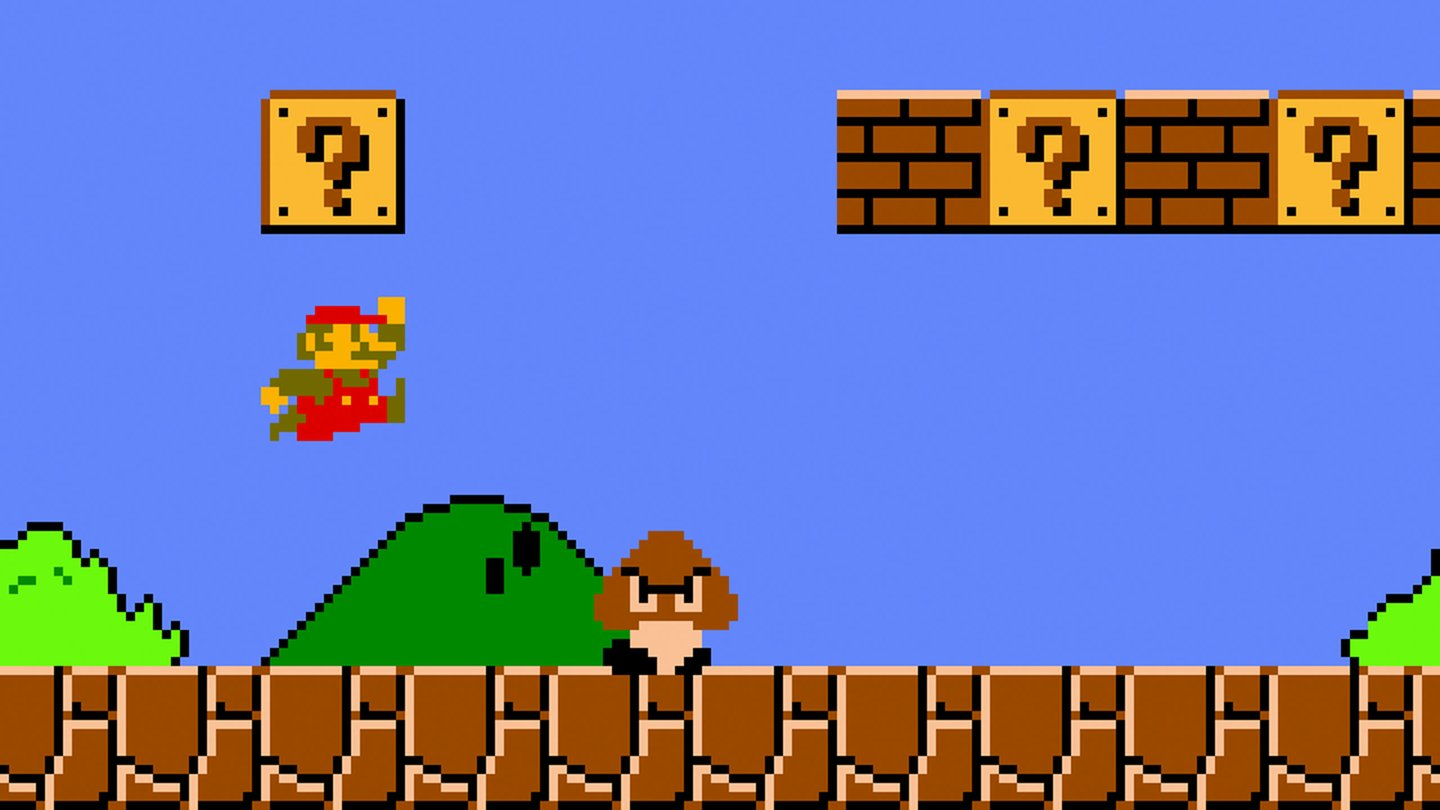
\includegraphics[width=\textwidth]{images/super_mario}
	\caption{A screenshot of the iconic Super Mario Game. It shows all three
	artifacts of a game: The model (positions of blocks), the simulation (Mario
	jumping), and the representation (textures and \glspl{sprite}).}
	\label{fig:super_mario}
\end{figure}

\paragraph{Game Simulation}

The game simulation is a logical abstraction of a game. The simulation is
responsible to update the state of all relevant game objects to progress the
state of the game as a whole. In most games the game simulation is realized with
a physics engine along with a game logic that steers the simulation.

\paragraph{Game Presentation}

The game presentation is responsible for rendering the game state on the player
device's screen. Changes in the game state must be made visible by the game
presentation as soon as possible.

Game simulation is usually tightly coupled with the game presentation. This is
due to the nature of the most basic graphics libraries like DirectX or OpenGL
which are the foundation of most video games. These graphic libraries typically
have one main render loop. Within this loop the developer gets a chance to apply
input to every game object before it is drawn to the screen. As a consequence
the game simulation cannot be completely separated from the presentation
process. The book Real-Time Rendering \cite{RTR3} is a good reference for
graphics libraries. Furthermore the web-page of the book provides a
comprehensive selection of related literature and technical examples.

\paragraph{Game Model}

The game model consists of a meta model containing a set of object types and a
physical model which is an instantiation of the meta model representing the game
state. The game simulation operates upon the game state to progress the game.
Static data like for example audiovisual information like textures, model, or
sound files which are only used for the game presentation and not for the
simulation are directly stored in the meta model. Static data can be referenced
by the presentation as needed.

\subsubsection{Game Engines}
All the artifacts of a game as described in the previous three sections are
fairly low level. To relieve the developer from the need to cope with these low
level artifacts game engines are used. Game engines come with comprehensive
editors, tools and libraries to abstract complex low level functionality to
allow developers to focus their effort on the core parts of the game.

\subsubsection{\ogs{}}
\ogs{} are a special case of traditional video games. In addition to the
audiovisual representation the player not only interacts with the game
simulation but also with other players playing at the same time at another
location. \ogs{} introduce asynchronism to games which forces a completely
different application design in comparison with traditional single-player games.

\paragraph{Simple \ogs{}}

\begin{figure}
	\centering
	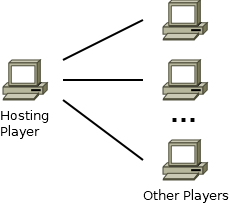
\includegraphics[width=5cm]{images/SimpleOnlineGame}
	\caption{In a simple \og{} one player hosts a game session and other players
	connect to it.}
	\label{fig:simple_online_game}
\end{figure}

Simple \ogs{} are very similar to single-player games with the addition that
some enemies or companions are played by other human players. In simple \ogs{}
players are responsible to set up the game's multi-player environment (hosting
the game session and connection to it). These can be client-server or
peer-to-peer scenarios. In any case one player is always responsible to host the
game (\autoref{fig:simple_online_game}). In simple online games the players have
full control over the game rules. This makes them comparable to classical board
games in a sense that all players agree to a set of rules. Cheating is therefore
not an issue most of the time.

Examples of such simple games are Quake, Age of Empires, or Diablo 2. Lately it
has become popular for simple \ogs{} to provide a matchmaking service that helps
players to find each other for game sessions. This matchmaking functionality is
responsible to initiate the game session on all clients but does nothing beyond
that. Hence the session is simulated locally on one of the clients. This client
has zero latency to the simulation and has therefore an advantage over the other
players. In this setting cheating clients are a common problem since the hosting
player can basically influence the game at will.

\newpage
\paragraph{Rich \ogs{}}

\begin{figure}
  \centering
  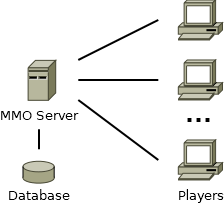
\includegraphics[width=.36\linewidth]{images/MMO}
  \caption{In an MMO environment all players connect to a single MMO server.}
  \label{fig:mmo}
\end{figure}
\begin{figure}
  \centering
  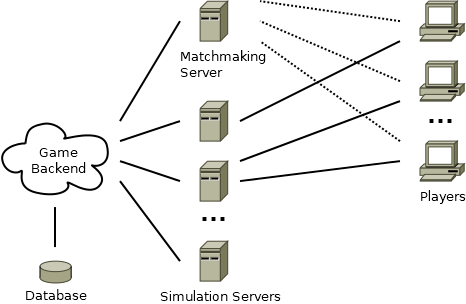
\includegraphics[width=.76\linewidth]{images/RichOnlineGame}
  \caption{Modern \og{} simulate game sessions on servers to provide the best
  player experience.}
  \label{fig:rich_online_game}
\end{figure}

While continuously gaining popularity simple \ogs{} also went through an
evolution. The most noticeable improvement is that modern \ogs{} often take the
control over the game environment away from the player. This means that the game
is simulated on a server environment and the local game client is only
responsible for the presentation of the game and for sending inputs to the
server. In this setup the game state is persisted on the server side in a
persistent storage. The persistence of the game state in this fashion allows for
a set of features which really separate today's \ogs{} from the classical simple
online or offline video games. These modern \ogs{} will be referred to as rich
\og{} in this thesis.

Rich \ogs{} are also very comfortable for the players. The players only need to
download the game client to play the game and are spared any environment setup.

The first occurrences of rich \og{} have been \glspl{mmo}. In \glspl{mmo} the
player controls an avatar in a persistent virtual game word playing against the
environment (monsters, traps, dungeons, \ldots) and other players (combat,
trading, chatting, \ldots). \glspl{mmo} are simulated using a single dedicated
server to simulate the whole game (see \autoref{fig:mmo}). This limits the
number of player who can simultaneously participate in the game\footnote{In the
very popular \gls{mmo} World of Warcraft the player number per server is
limeted to about 10'000 simultaneous players.}. \glspl{mmo} solve this problem
by adding or removing complete instances of the full game. But this approach
does not scale very well since player number can vary greatly.

Besides \glspl{mmo} many rich \ogs{} exist in various genres like: First Person
Shooters (Counter Strike, Battlefield, Overwatch), \gls{moba} games (League of
Legends, Dota 2), Sport Games (FIFA, NHL, Golf), Car Racing Games, and many
more. What all these games have in common is that they are simulated in a server
environment (\autoref{fig:rich_online_game} shows an example of such a server
environment). This setup allows for completely fair and cheat safe game
sessions. This solution provides the best possible experience for \ogs{}. The
drawback is that running the simulation services has considerable computing and
bandwidth requirements which can be very expensive.

\subsubsection{Procedural Content Generation}

\gls{pcg} has always been an integral part of game
development and has gained recent popularity because of prominent games that
make extensive use of \gls{pcg}. Some examples are Minecraft, Terraria
(\autoref{fig:terraria}), No Mans Sky to only name a few.

\begin{figure}
	\centering
	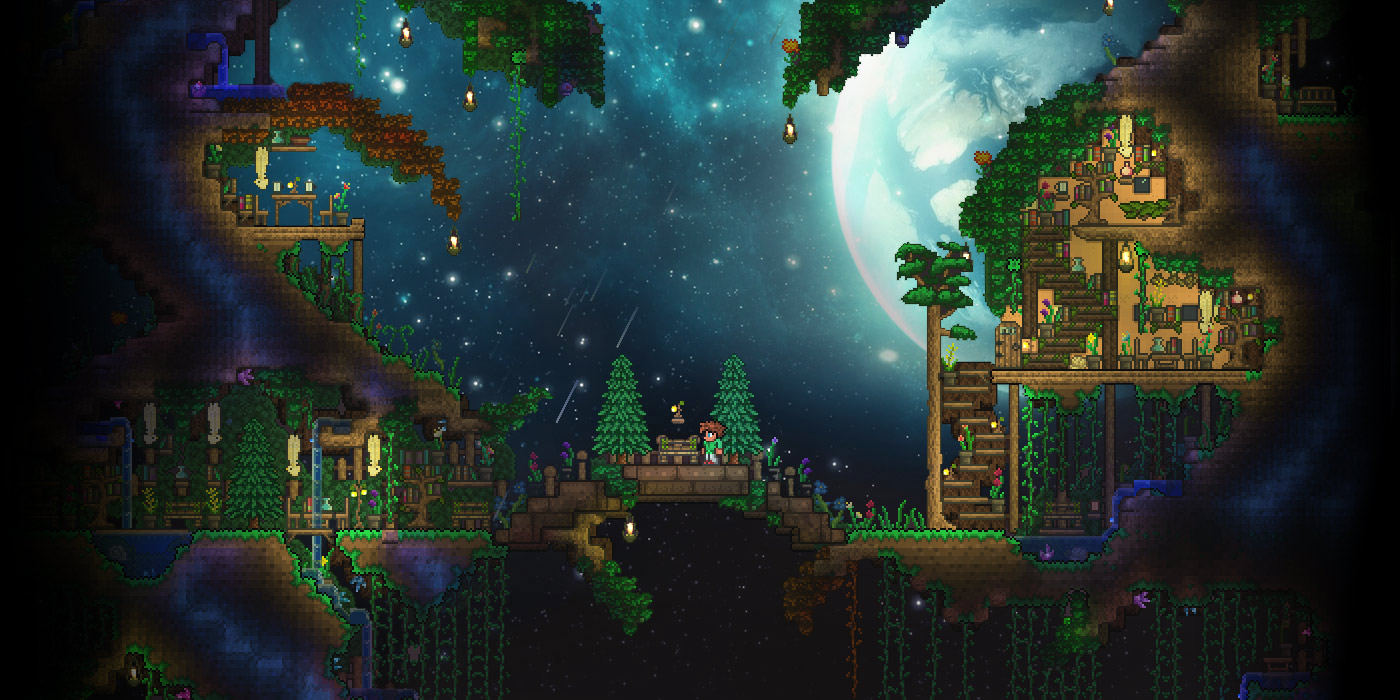
\includegraphics[width=\textwidth]{images/terraria}
	\caption{A screenshot of Terraria which makes intensive use of \gls{pcg}. The game
	world is different every time the game is played. This encourages
	replayability.}
	\label{fig:terraria}
\end{figure}

\gls{pcg} is the process of automatically generating game content. A canonical
example in this regard is vegetation generation. The developer only needs to
supply certain parameters like for example color distribution and branching
factor for trees. The game then creates all the vegetation before the game
starts or even dynamically while the game progresses as needed.

\gls{pcg} also allows generate levels, quests, weapons, vehicles, and even
sounds. A good reference for \gls{pcg} is the book Procedural Content Generation In
Games \cite{shaker2014procedural}. It contains many useful \gls{pcg} methods and
gives a good overview on the topic.

\subsection{\mss{}}

\mss{} are an implementation approach for a \glsreset{soa}\gls{soa}
\cite{zimmermann2016microservices}. In \gls{soa} an application is decomposed
into logical units that each solve one specific task. In a \ms{} application
each of these units is represented by a service that runs in an isolated
process. A service is usually deployed in a container which supports isolation
and simple replaceability. The services communicate over a lightweight shared
inter process communication channel respecting the smart endpoints - dump pipes
principle. C.Richardson's article ``Microservices: Decomposing Applications for
Deployability and Scalability'' \cite{richardson2014mss} is a good introduction to
\mss{}.

Over the years many discussion about the differences and similarities between
\gls{soa} and \mss{} took place \cite{little2017soaVSms},
\cite{ogradly2017soaVSms}, and \cite{little2015soaVSms}. In his article ``The
Difference between \gls{soa} and Microservices?'' M.Little collects arguments of
experts in the \ms{} scene like D.North \cite{north2015mss} and
J.Stenberg\cite{stenberg2014mss}. One trend that he highlights is that \gls{soa}
is loosing popularity and \mss{} are gaining popularity. One reason for this
could be that \gls{soa} is mainly a vendor driven effort whereas the \ms{}
approach is driven far more by developers as he states. Also the success of
\ms{} friendly platforms like AWS indicate that service driven platforms are an
effective way of building applications that are resilient and scalable.

\subsubsection{\ms{} Tenets}

In O.Zimmermann's article \ms{} tenets he provides seven \ms{} tenets to
describe the properties of \ms{} applications
\cite{zimmermann2016microservices}. According to the tenets a correlation
between game specific requirements and \ogs{} can be made. In the course of this
thesis a selection of the \ms{} tenets will be used as an indicator to show
that \mss{} are suitable to drive \og{} applications.

The remainder of this section will give a brief overview over all \ms{} tenets
that are relevant for this thesis.

\paragraph{Fine-grained Interfaces and Single Responsibility}

Every \ms{} should offer all of its functionality in the form of a fine grained
interface that decouples the service implementation from its interface. This
interface is usually exposed via REST/HTTP and is accessible via a reverse
proxy. Each \ms{} should only have one responsibility in regards to the domain.
This allows services to be independently deployed, changed, replaced and scaled.

\paragraph{Domain-Driven-Design}

The responsibility of a \ms{} should be derived from the problem domain, and
each service should be dedicated to exactly one aspect of the domain. If one
domain aspect is very extensive it can lead to a large \ms{} which is not
desirable. This can be an indicator that the granularity of the services might
be wrong. Granularity is the most challenging part of \gls{ddd}
\cite{millett2015patterns}.

\paragraph{IDEAL}

The IDEAL tenet is a collection of cloud patterns. These patterns do partially
overlap with several other tenets like single responsibility or decentralized
continuous delivers. None the less this tenet is a great indicator to
evaluate if an application respects the major cloud principals. C. Fehling et
al. provide a good overview over the  IDEAL Cloud Application Properties
which is summarized in this section \cite{fehling2015cloud}.

\subparagraph{Isolated State}
A \ms{} should be stateless which means that a request that is sent to a \ms{}
should be completely confined in itself. As a consequence \mss{} are not allowed
to store date in-memory between requests. Instead the state should be stored in
a persisted data storage provided by the cloud e.g. another \ms{}.

\subparagraph{Distribution}
To allow an application to scale, its functionality is spread out among several
different \mss{}. These shards are then deployed in cloud environments which are
large distributed systems themselves. \ms{} applications are a natural match for
the distributed nature of cloud environments.

\subparagraph{Elasticity}
Elasticity inquires if the application can be scaled during operation. When
the need of scaling arises it must be possible to add and remove \ms{} instances
without affecting the stability of the whole system.

\subparagraph{Automated Management}
In order to quickly react to scaling demands or to recover from failure the
management approach to these scenarios should be fully automated.

\subparagraph{Loose Coupling}

The dependencies among \mss{} should be reduced as much as possible. It is not
feasible to reduce dependencies to zero because without any dependencies the
application is not able to function as a whole unit. The goal is to keep the
amount of dependencies low in order to keep the impact of adding and removing
new functionality at a minimum.

\paragraph{Polyglot Programming and Persistence}

The polyglot tenet is the main driver when it comes to \ms{} confinement. It
states that a \ms{} has no restriction on storage paradigms and implementation
details. As a consequence each \ms{} can be designed in a way that best suits
its purpose.

Polyglot persistence is especially crucial for \ms{} applications. The classical
approach of having one big database for the whole application is called an
integration database and is an anti-pattern for \mss{} since it introduces a
single point of failure. With polyglot persistence each \ms{} can use the
storage paradigm that is best suited for it. This eliminates the need for a
central persistence solution and therefore the single point of failure.

Polyglot programming allows development teams to work with the languages and
tools that they are used to. This greatly speeds up the development process. It
also allows to integrate arbitrary technology into the application like for
example legacy systems.

\paragraph{Lightweight Containers}

Lightweight containers are an enabling technology for \ms{} applications.
Containers allow to build each \ms{} in its own confined environment. Containers
guarantee that the \ms{} runs with the identical configuration despite a
different run-time environment (developer PC, build and test server, cloud
provider infrastructure).

Containers allow for easy deployment and scaling of a \ms{} application. They
also allow rolling updates which means that a part of the application can be
exchanged without interrupting the operation of the application.

\paragraph{Decentralized Continuous Delivery}

Continuous delivery is the ability to extend an existing \ms{} application which
is already in production. The main goal is to facilitate the delivery of
extensions safely, quickly and regularly. Decentralized in this regard means the
absence of a central artifact that has to be delivered every time the
application changes.

\paragraph{DevOps}

DevOps engineers are the glue between the development and the operation of a
\ms{} application. The idea is that DevOps engineers are already part of the
project during the initial development of an application and remain responsible
for the application after it's release. This gives the DevOps of to a certain
application a deep understanding of it's technical requirements. DevOps are also
responsible to test the deployment process early to guarantee a smooth
transition to the production life-cycle of an application. When a \ms{}
application is in production the DevOps engineers have enough insight into the
application internals to be able co cope with most problems that arise in the
long term. A. Earnshaw published a blog-post that describes DevOps very
well \cite{earnshaw2013devops}.

\subsubsection{\ms{} Composition}
\label{subsub:composition}

\ms{} composition is a very wide term and therefore needs to be further
specified. For this purpose large domain composition can be split into two sub
topics which are suited to be examined separately: physical composition and
logical composition.

\ms{} composition can be categorized into two composition paradigms:
Orchestration and Choreography \cite{varjoinen2014orchestrationVSchoreography},
\cite{lublinsky2008orchestrationVSchoreography}. Orchestration states that a set
of \mss{} is composed by a central intelligence unit which is responsible for
the management the application \cite{cohen2015orchestration}. Choreography
implies that there is no central intelligence and the cluster of \mss{} as a
whole is responsible to guarantee the stability of the application
\cite{millidge2015choreography}, \cite{vilas2016choreography}, and
\cite{jellema2017choreography}.

\paragraph{Physical Composition}

Physical composition is the discipline to bring a set of \mss{} onto a
physical computing environment, usually the cloud. In the case of the cloud the
term physical is understood as the appropriation of computing, memory, disc
space and networking capabilities. In a cloud setting these physical
requirements are covered by using a \gls{paas} solution
\cite{lawton2008developing}, \cite{buyya2009modeling}.

Physical composition is usually enabled using composition engines like for
example docker-compose, docker-swarm, Apache Mesos or Kubernetes. The majority
of the composition engines use an orchestration approach. 

\paragraph{Logical Composition}

Logical composition is the aspect of how a set of confined \mss{} is working
together to solve the goal of the application as a whole. There is no
general solution for logical composition, which is why the developers of an
application have to cope with this task themselves.

Logical composition of a \ms{} application has two major requirements that must
be satisfied. The services have to know how to find each other
\cite{rotter2017telecom} and the services must be aware of the communication
semantics \cite{oberhauser2016microflows}.

Usually logical composition is realized with an RESTful \gls{api} description
that can be accessed via a \gls{http}. Especially for regular web applications a
vast choice of middle-ware is available, for example Swagger, JaxRS, JSON API,
and API Blueprint just to name a few.

The composition paradigm (Orchestration or Choreography) that is used for
logical composition is strictly dependent on the type of application under
development. In an orchestration solution there would be one central point where
\mss{} could look up crucial information like message formats and service
locations. In a choreography solution this information would be distributed
among all services to form a mesh of information about the application cluster.
In this case information can be requested from any \ms{} in the system.

\subsubsection{\ms{} Deployment}

\ms{} deployment comprises the whole process that is necessary to bring an
application from the development stage into production. This process includes
several steps:

\begin{itemize}
  \item Bring the application code along with eventual dependencies into the
  service containers
  \item Upload the application containers to the cloud
  \item Prepare the application on the cloud side
  \item Start the application as a whole by starting all service containers
  \item Scale the application according to operational needs
  \item Set up backup and recovery solutions for the application
  \item Deploy a monitoring solution to keep track of the application
\end{itemize}

While most of these processes can be automated in the long term it requires a
lot of effort to bring these deployment automation procedures into place.

\subsubsection{\ms{} Development}

\ms{} development consists of the whole process of designing an application
using an approach suited for \ms{} development. This includes writing the code
for the application and to manage the collaboration of different developers on
the same project.

\section{Delimitations and Assumptions}

This section lists several limitations which had an influence on this
thesis.

\subsection{\mss{} are Developed by Teams}
One of the greatest advantages of \mss{} is that they allow to split the
development of a complex application into small shards that can be developed by
small flexible individual teams \cite{anderson2017teams}. This aspect of \mss{}
can only be analyzed conceptually because this thesis is a one-man project.

\subsection{Zero Budget}
\label{sub:zero_buget}
Cloud service providers like Amazon or Google offer a free tier to evaluate
their cloud capabilities. But even these free tiers of subscription require a
valid credit card in case the free quota is exceeded. This is a risk that
\gls{hsr} did not want to bear. As a consequence the target environment for this
thesis is a virtual server provided by \gls{hsr}. This setup makes it difficult
to finalize the process of game development with \mss{} because in a real world
example companies would rely on cloud service providers to have a stable cloud
computing environment. It is also a pity because both Google and Amazon have
just recently released dedicated solutions for the deployment of \ogs{} on their
environments. Evaluating these solutions would have been a very interesting
topic.

\subsection{Limitations Introduced by Video Games}
As explained in \autoref{sub:games} the way video games are built themselves is
a huge limitation on the design of an \og{} application. To analyze all problems
which occur in this regard is out of scope for this thesis. Instead this thesis
takes a more general approach by viewing the rendering and physic engine
details as a black box. This allows to focus on the interesting parts of \og{}
development, the game model and the game simulation, which is most relevant in
regards to a \ms{} realization.

\subsection{Time Constraint}
In the original plan for this thesis the topic \glsreset{pcg} \gls{pcg} was
intended to be researched in greater detail. But since the topics deployment and
composition required a lot more effort than anticipated, the time budget for
\gls{pcg} shrunk close to zero. Because of this \gls{pcg} will only receive
minor attention in this thesis.

Another aspect that intensified the time constraint is the fact that this thesis
is the third out of a series of three and a lot of effort was necessary to
conclude the project as a whole.

\subsection{Operating System Delimitation}
\label{sub:delimitations}

Games are usually developed using Microsoft Windows because it offers the
largest ecosystem for game developers \cite{bolas2013games_dev_windows}. But my
impression is that cloud developers mainly tend to use Linux tools. Because of
this many tools are cumbersome to use on Windows platforms and therefore greatly
hinder the development process. It is a side-goal of this thesis to facilitate
the whole process on Windows in a more satisfactory way.\\





















